\subsection{(W) Slalom}\label{s:testSlalom}
    \noindent TODO:
        \begin{itemize}
            \item Main goal: static obstacle avoidance, open space navigation, determinism of the avoidance run in addition to obstacle avoidance
            
            \item hidden waypoint.
            \item \emph{Open space obstacle} (fig. \ref{fig:slalomOpenSpaceObstacle}) - avoidance of open space obstacle, while tracking \emph{hidden waypoint}.
            
            \item \emph{Hidden waypoint navigation} is shown in three stages start (fig. \ref{fig:slalomHiddenWaypointStart}), middle (fig. \ref{fig:slalomHiddenWaypointMiddle}), and end phase (fig. \ref{fig:slalomHiddenWaypointEnd}).
            
            \item there is multi-variability in path selection, because waypoint is reachable by various cost-equivalent path
            
            \item right down strategy is preffered from UAS POV
        \end{itemize}
    
    
    The \emph{standard test setup} defined in (tab.  \ref{tab:testMovementOrientations}. \ref{tab:testUASBasicParameters}. \ref{tab:testNavigationGridBasic}. \ref{tab:testAvoidanceGridBasic}. \ref{tab:testUASColoring}) is used with following parameter override:
    \begin{enumerate}
        \item \emph{Avoidance grid - type} - \emph{ACAS-like} with enabled \emph{Horizontal maneuvers}
    \end{enumerate}

    \begin{figure}[H]
        \centering
        \begin{subfigure}{0.48\textwidth}
            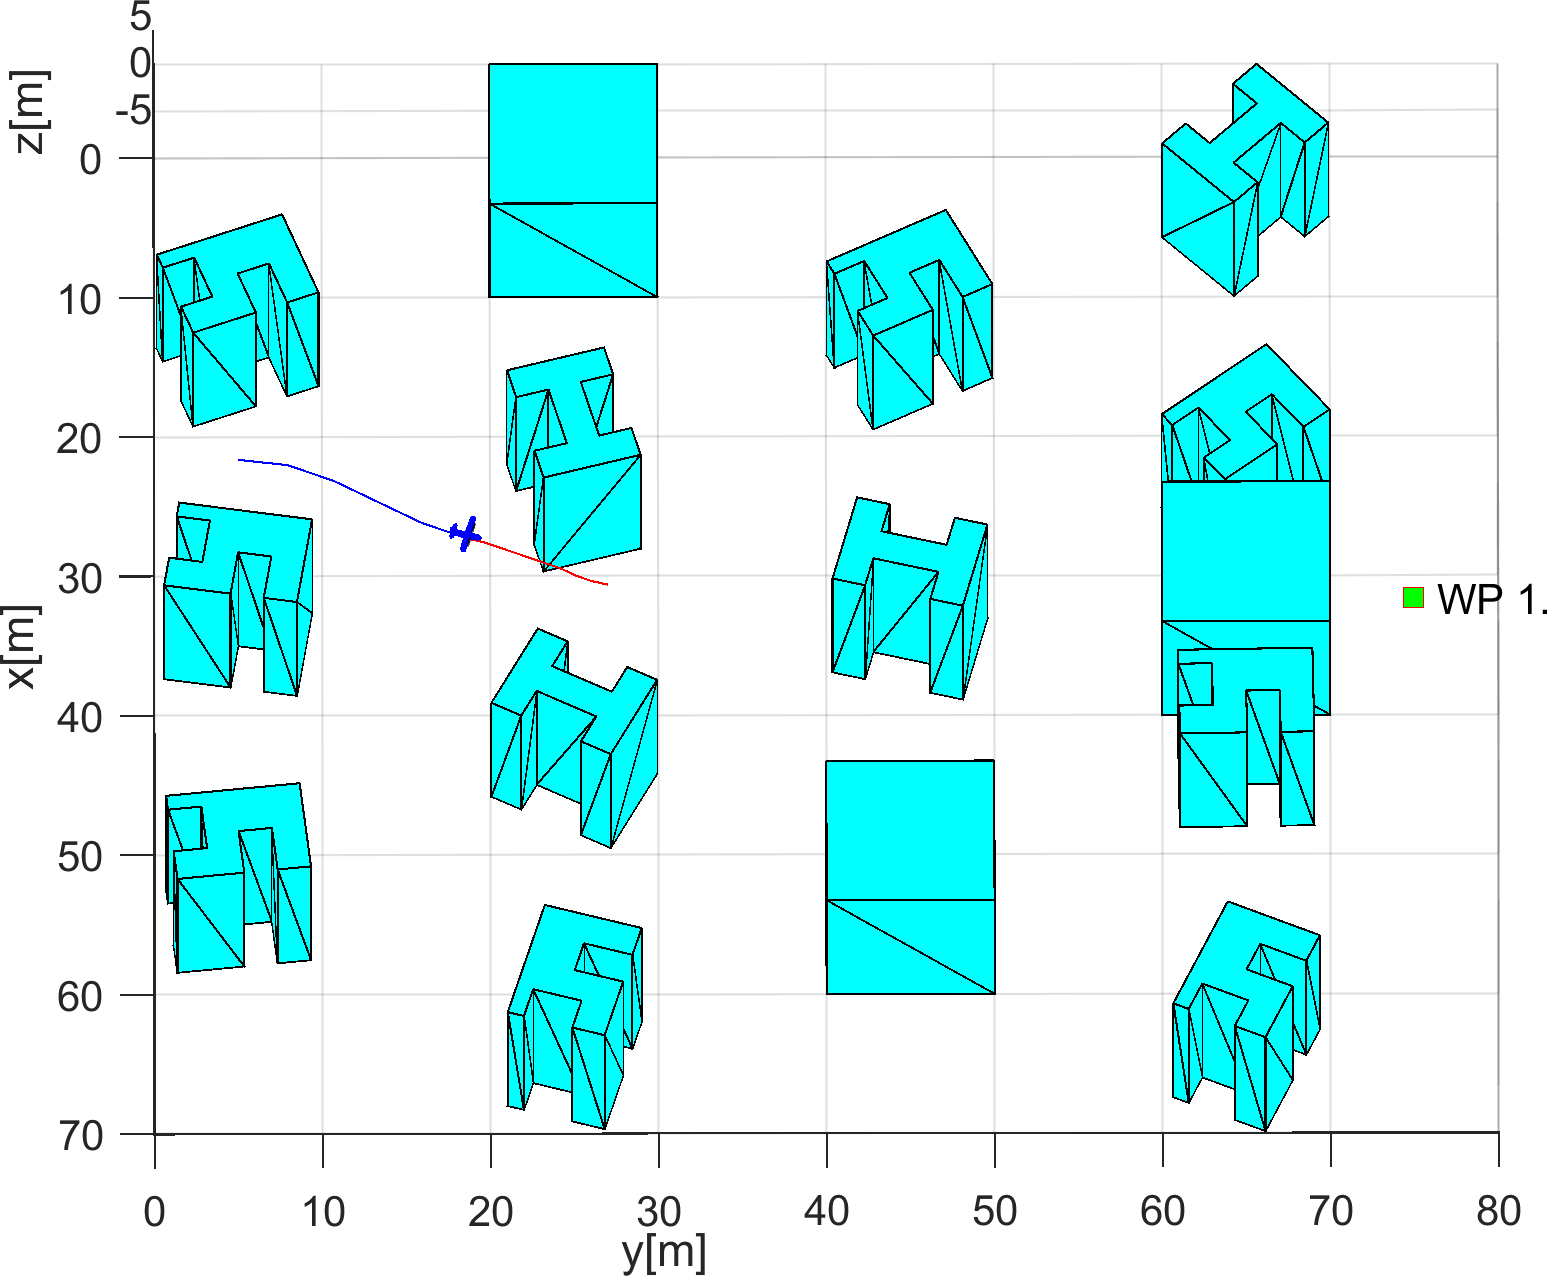
\includegraphics[width=0.9\linewidth]{\FIGDIR/NS007ConstraintsPolynomialSlalom-00015}
            \caption{Open space obstacle.}
            \label{fig:slalomOpenSpaceObstacle}
        \end{subfigure}
        \begin{subfigure}{0.48\textwidth}
            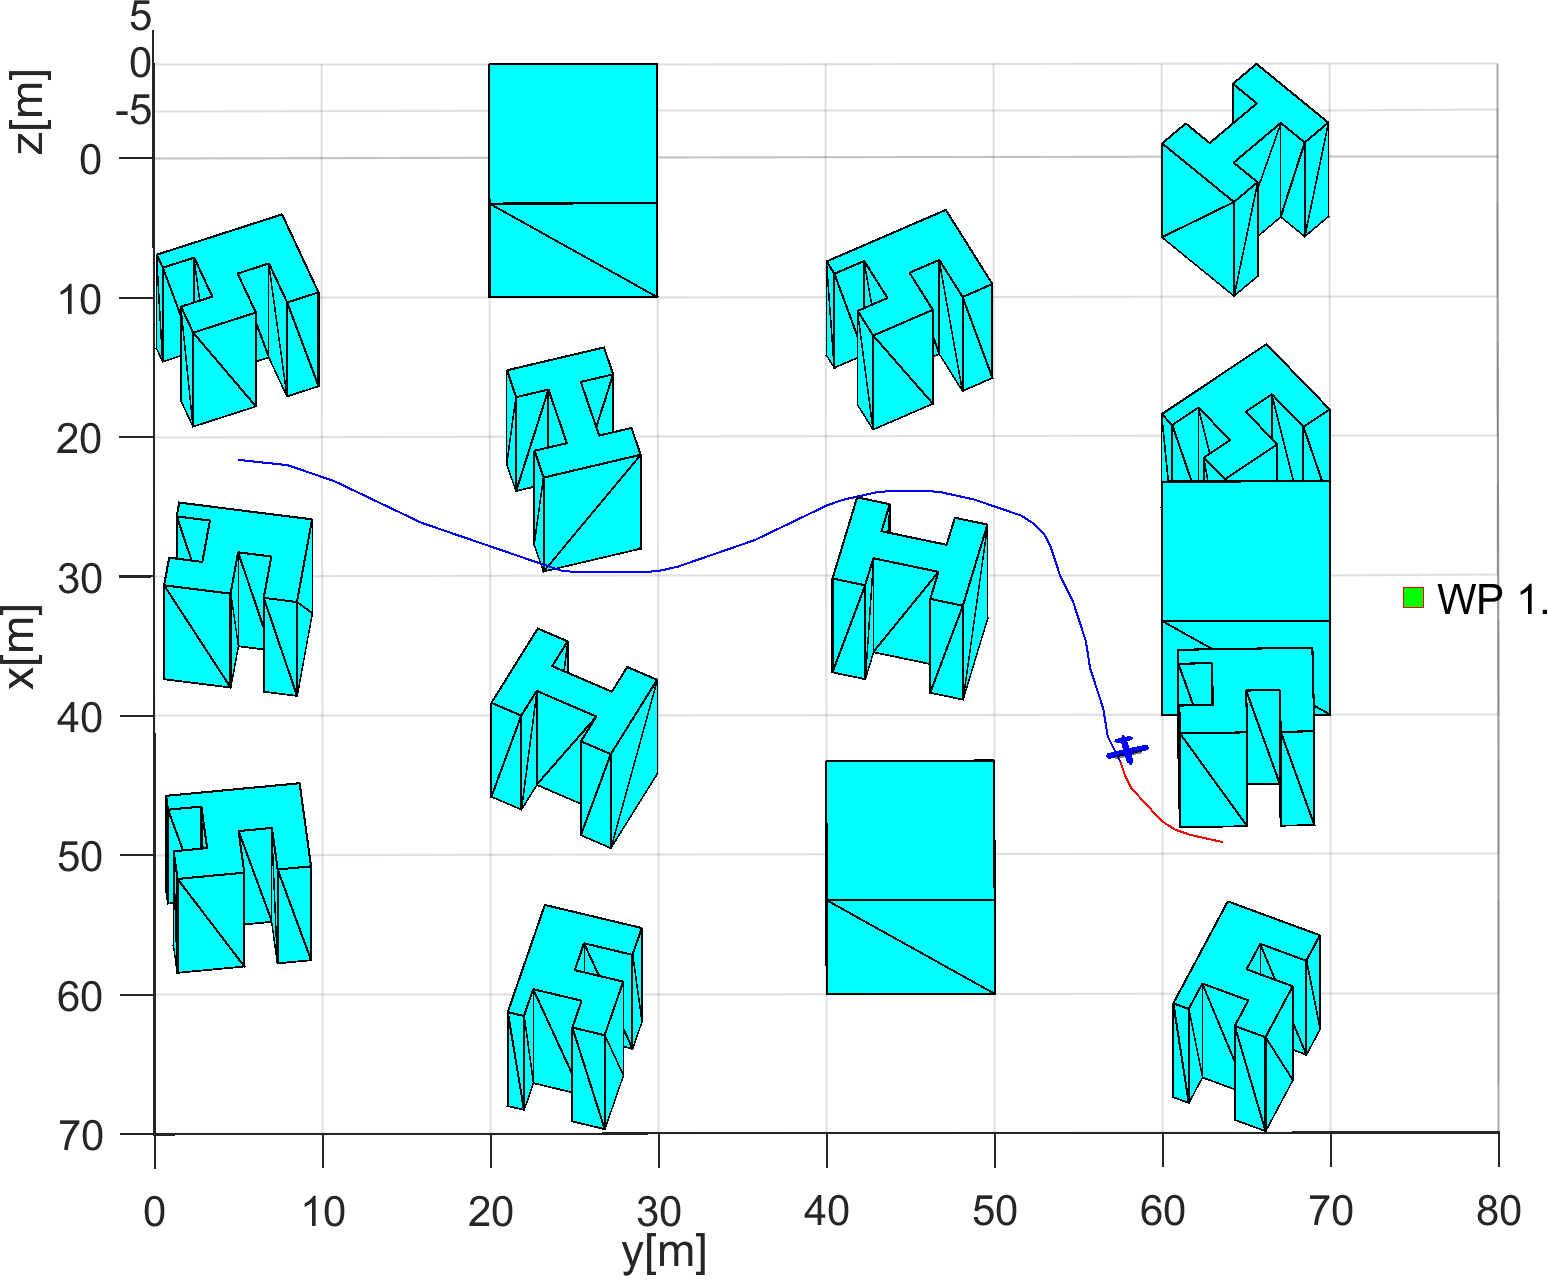
\includegraphics[width=0.9\linewidth]{\FIGDIR/NS008ConstraintsPolynomialSlalom-00069} 
            \caption{Hidden waypoint start.}
            \label{fig:slalomHiddenWaypointStart}
        \end{subfigure}
        \\
        \begin{subfigure}{0.48\textwidth}
            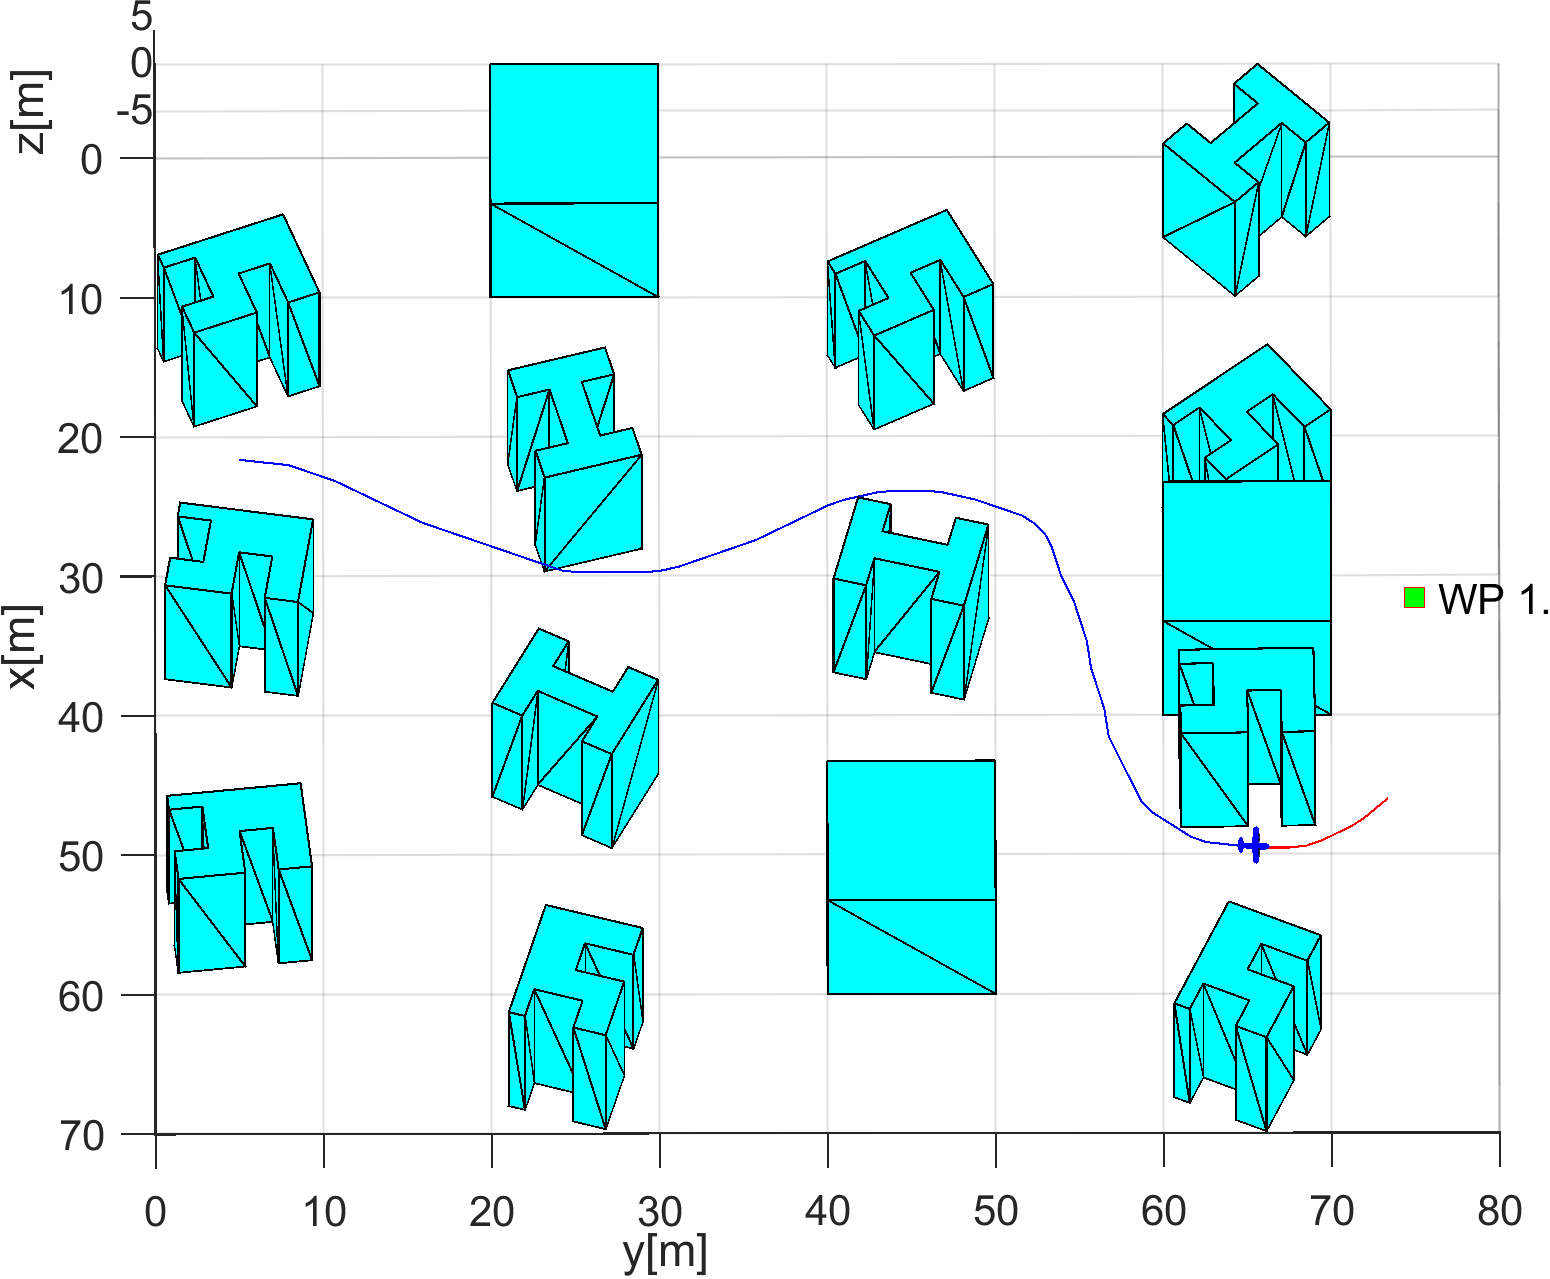
\includegraphics[width=0.9\linewidth]{\FIGDIR/NS009ConstraintsPolynomialSlalom00080} 
            \caption{Hidden waypoint middle.}
            \label{fig:slalomHiddenWaypointMiddle}
        \end{subfigure}
        \begin{subfigure}{0.48\textwidth}
            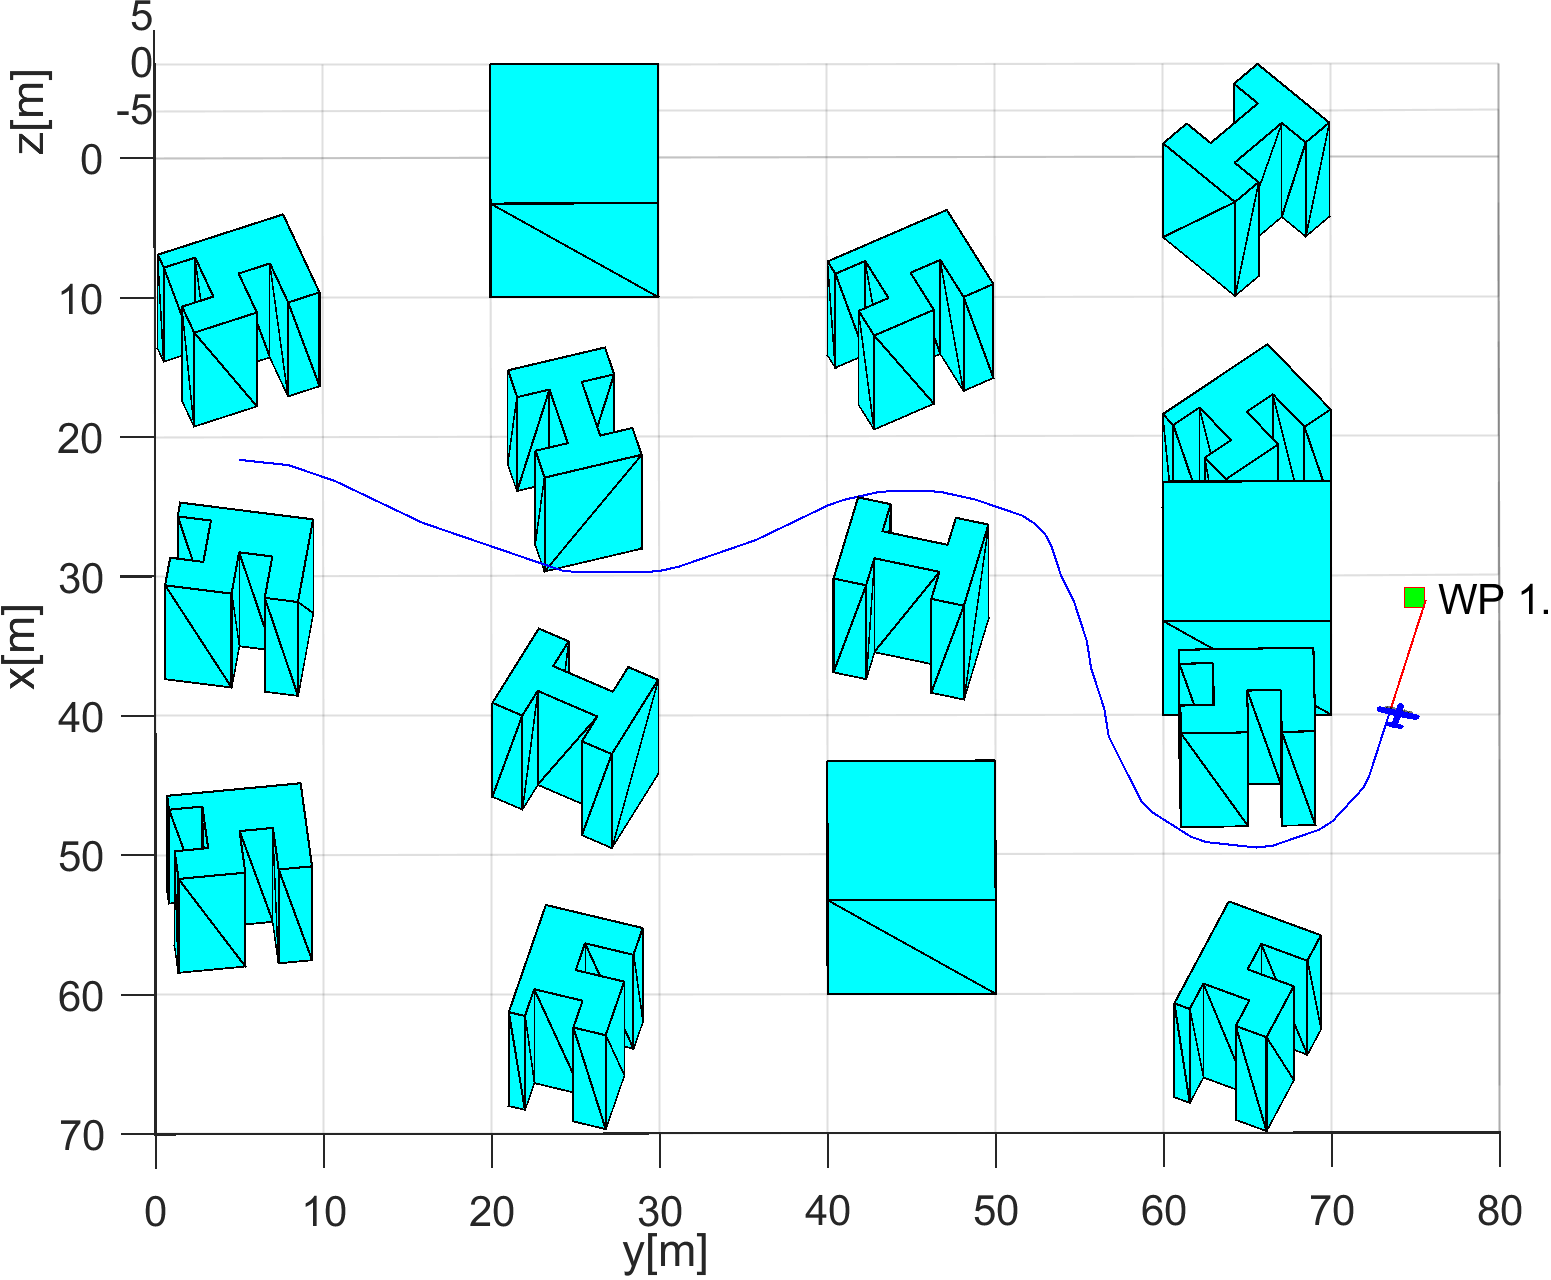
\includegraphics[width=0.9\linewidth]{\FIGDIR/NS010ConstraintsPolynomialSlalom00094} 
            \caption{Hidden waypoint end.}
            \label{fig:slalomHiddenWaypointEnd}
        \end{subfigure}
        \caption{Test scenario for \emph{Slalom} with \emph{hidden waypoint}. }
        \label{fig:testCaseSlalomwithHiddenWaypoint}
    \end{figure}
    
    
    \begin{table}[H]
        \centering
        \begin{tabular}{c|c||c}
            \multicolumn{2}{c||}{Position} & \multirow{2}{*}{$\mathscr{WP}_1$} \\\cline{1-2}
            $[x,y,z]$           & $[\theta,\varpi,\psi]$           & \\\hline\hline
            $[25,5,0]^T $        & $[0^\circ,0^\circ,90^\circ]^T$    & $[35,75,0]^T$        \\ 
        \end{tabular}
        \caption{Mission setup for \emph{Slalom} scenario.}
        \label{tab:missionSetupSlalomScenario}
    \end{table}
    
    
    \begin{table}[H]
        \centering
        \begin{tabular}{c|c|c|c|c|c}
            \multicolumn{2}{c|}{Obstacle} & \multicolumn{3}{c|}{Body Margin} & \multirow{2}{*}{Safety Margin}\\\cline{1-5}
            position & type & min. & max. & avg. &   \\\hline\hline
            multiple (4) & hospital & $[0.5,1]$ & $[2.2,3.1]$ & $[1.5,3]$  & $[1,3]$ \\\hline 
            multiple (7) & unusual  & $[0.3,1]$ & $[2.3,3.5$] & $[2,3]$  & $[1,4]$ \\\hline
            multiple (3) & square   & $[3,4]$   & $[4,5]$     & $[4,5]$ & $[1,4]$   \\
         \end{tabular}
        \caption{\emph{Obstacle set} for \emph{Slalom} scenario.}
        \label{tab:obstacleSetSlalom}
    \end{table}
    
    
    \begin{figure}[H]
        \centering
        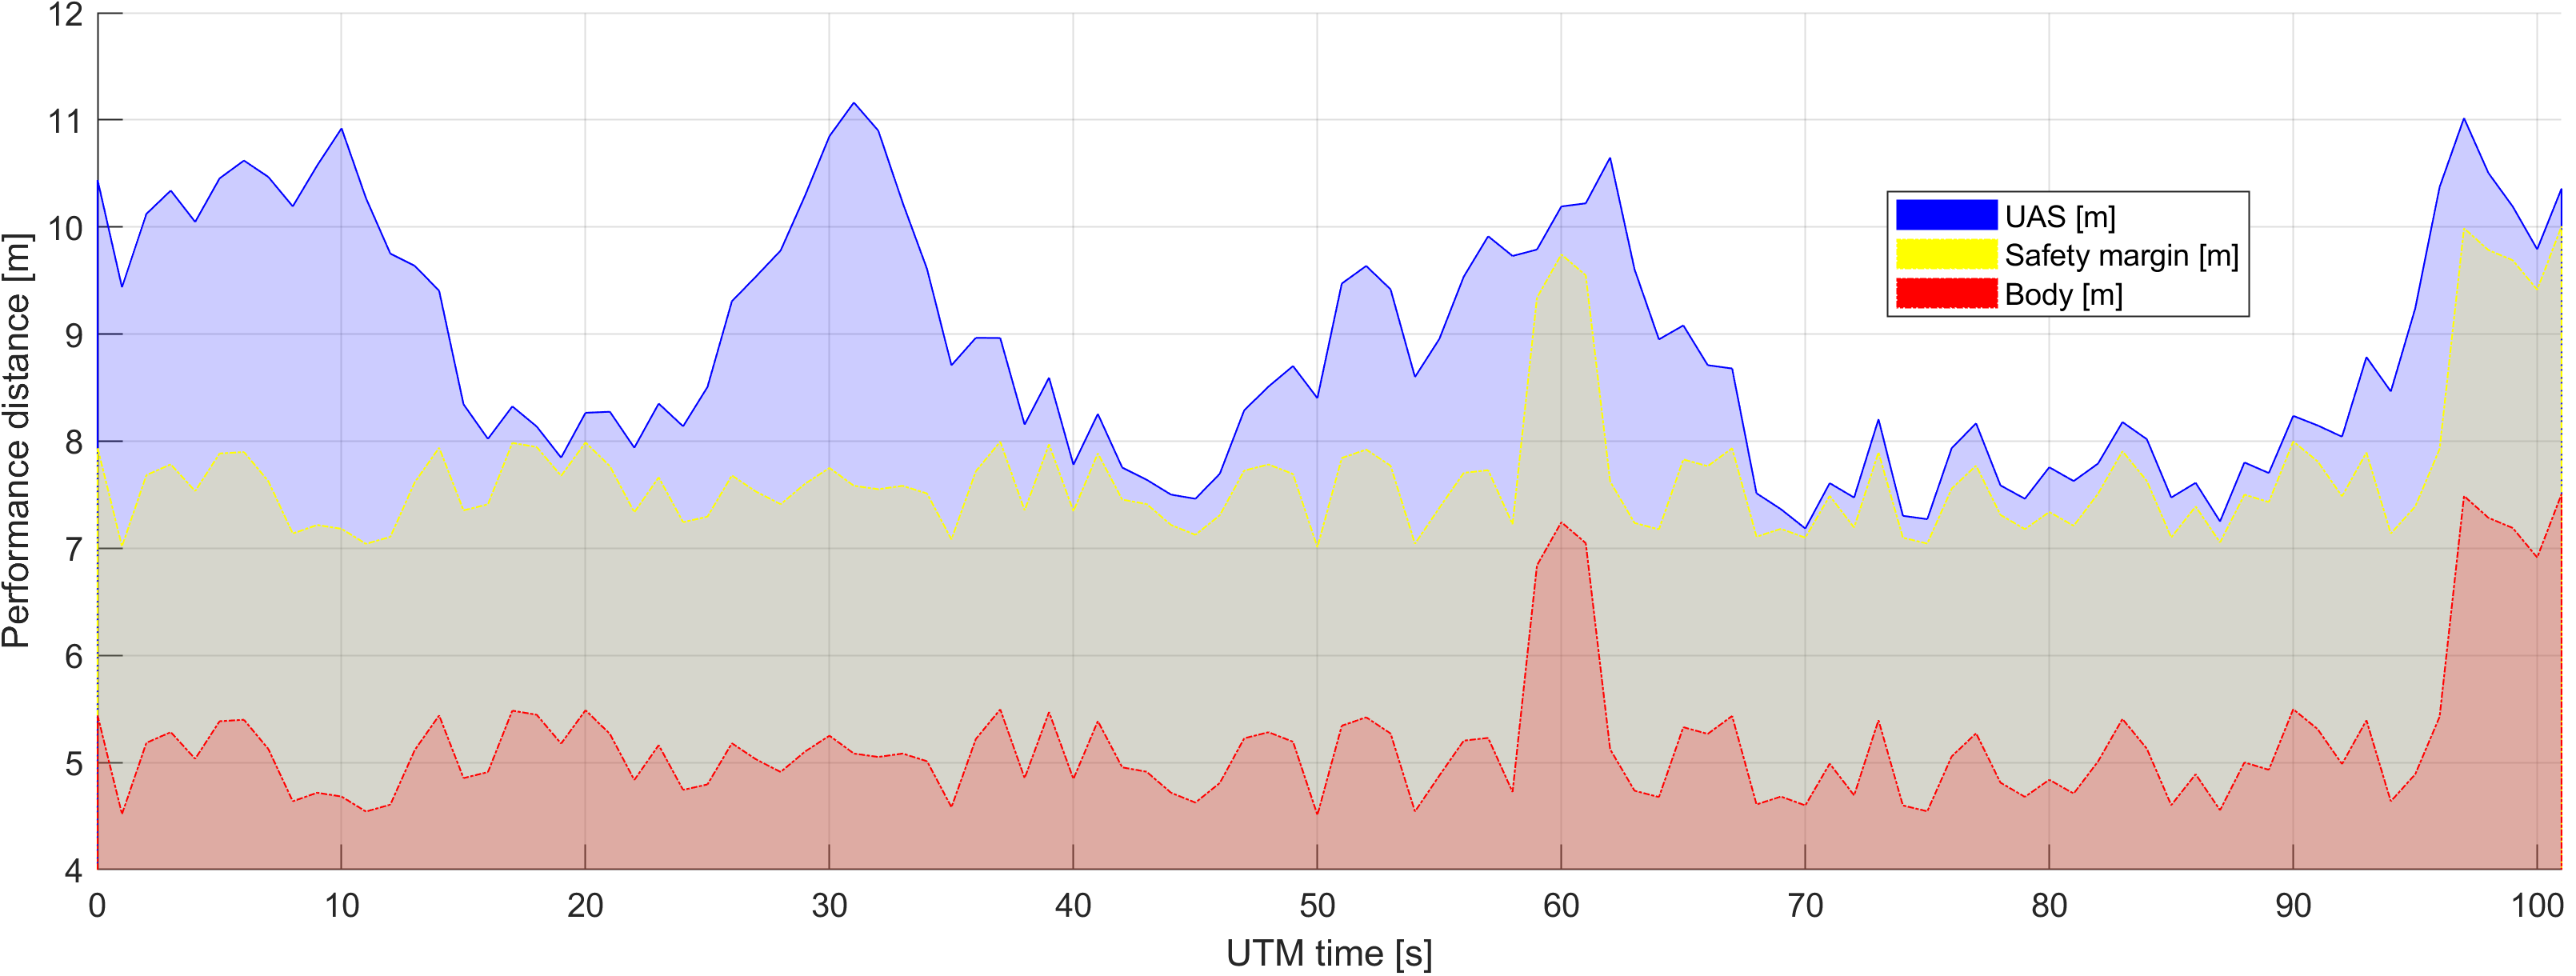
\includegraphics[width=0.8\linewidth]{\FIGDIR/NS011ConstraintsPolynomialSlalomPerformance} 
        \caption{\emph{Slalom} safety margin performance.}
        \label{fig:testCaseSlalomAvoidancePerformance}
    \end{figure}
    
    
    \begin{table}[H]
        \centering
        \begin{tabular}{c|c||c}
        \multicolumn{2}{c||}{Parameter} & UAS 1 \\\hline\hline
        \multirow{2}{*}{safety margin distance} & min & 0.0856\\\cline{2-3}
                                                & max & 3.7391 \\\hline
        \multirow{2}{*}{body margin distance}   & min & 2.5856  \\\cline{2-3}
                                                & max & 6.2391 
        \end{tabular}
        \caption{\emph{Slalom} safety and body margin distances.}
        \label{tab:testCaseSlalomSafetyAndBodyMarginDistances}
    \end{table}
    
    
    \begin{figure}[H]
        \centering
        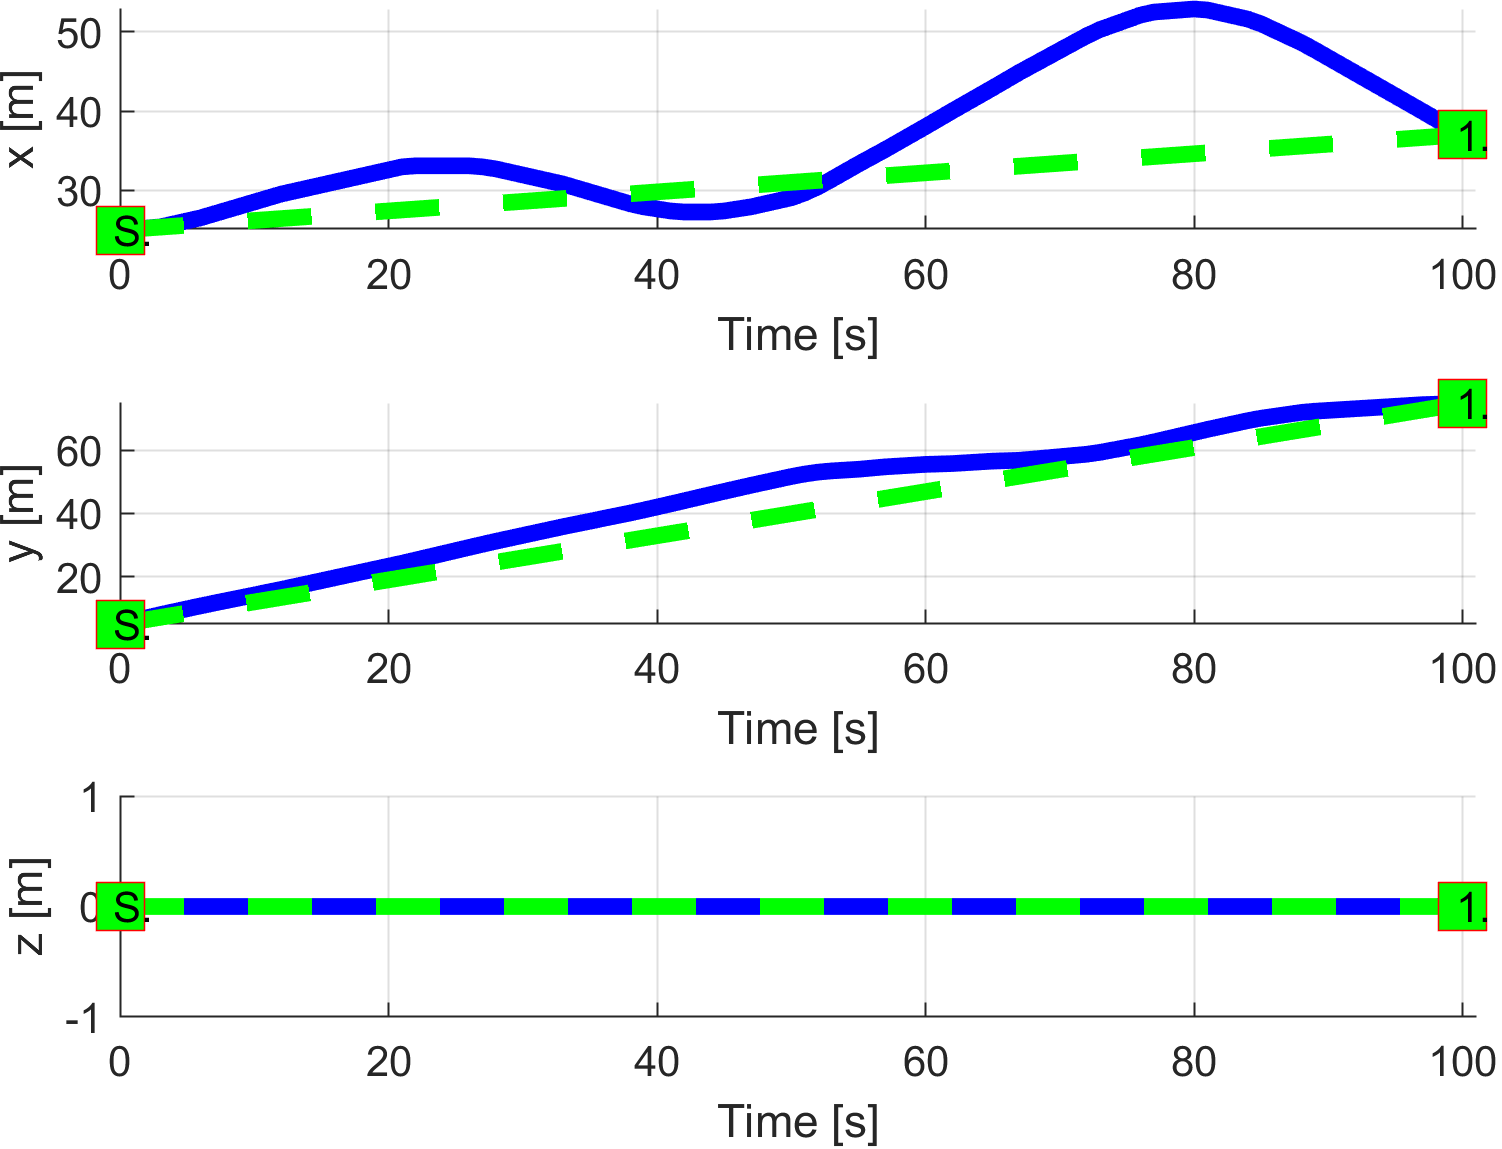
\includegraphics[width=0.55\linewidth]{\FIGDIR/NS012ConstraintsPolynomialSlalomPathFollowing} 
        \caption{\emph{Slalom} path tracking.}
        \label{fig:testCaseSlalomPathTracking}
    \end{figure}
    
    
    \begin{table}[H]
        \centering
        \begin{tabular}{c||c}
            \multirow{2}{*}{Param.} & UAS 1\\\cline{2-2}
                            & $\mathscr{WP}_1$  \\\hline\hline
              $\max |x|$    & 17.90      \\\hline
              $\max |y|$    & 12.41    \\\hline
              $\max |z|$    & 0        \\\hline
              $\max dist.$  & 20.06   \\
        \end{tabular}
        \caption{Path tracking properties for \emph{Slalom} scenario.}
        \label{tab:pathTrackingParametersForSlalomAvoidance}
    \end{table}
    
    
